The system scale, measured in number of cores, has a direct impact on the failure rate seen by the application. To study its impact, we varies $N$ from 10,000 to 1,000,000 with $W$ scaled proportionally, i.e., $W=N$. When MTBF is 5 years, the results are shown in Figure~\ref{fig:n5}. Please note that the time and energy for checkpointing when $N=1,000,000$ are beyond the scope of the figures, so we mark their values on top of their columns. When completion time is considered, Figure~\ref{fig:nt5} clearly shows that each of the three fault tolerance alternatives has its own advantage. Specifically, checkpointing is the best choice for small systems with around 10,000 cores, Lazy Shadowing outperforms others for systems with around 100,000 cores, while process replication has slight advantage over Lazy Shadowing for larger systems. On the other hand, Lazy Shadowing wins for all system sizes when energy consumption is the objective. 

When MTBF is changed to 25 years, the performance of checkpointing improves a lot, but is still much worse than that of the other two approaches. Lazy Shadowing also benefits from the increased MTBF, and further reduces its completion time and energy consumption. Specifically, Lazy Shadowing is able to achieve shorter completion time than process replication when $N$ reaches 1,000,000.

\begin{figure}[!t]
	\begin{center}
		\subfigure[Expected completion time]
		{
			\label{fig:nt5}
			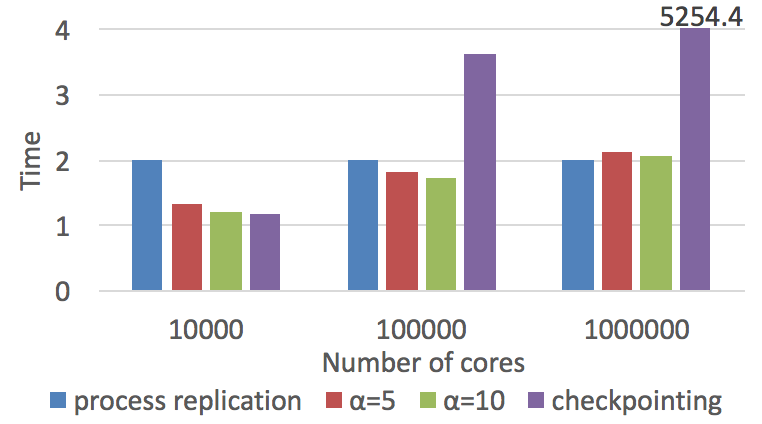
\includegraphics[width=0.7\columnwidth]{Figures/tnt5}
		} 
		\subfigure[Expected energy consumption]
		{
			\label{fig:ne5}
			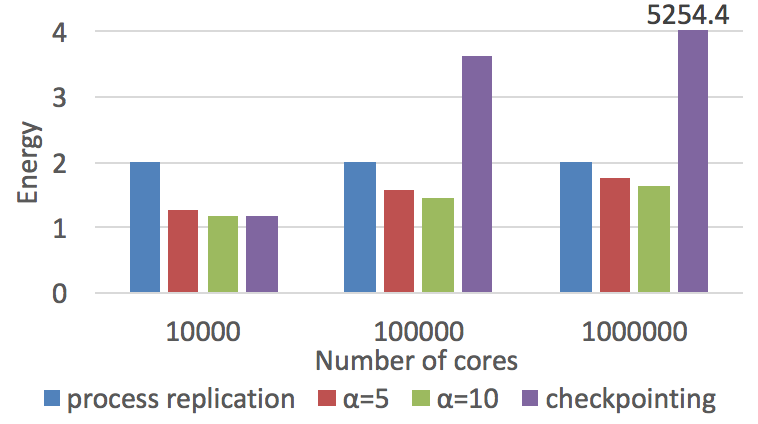
\includegraphics[width=0.7\columnwidth]{Figures/tne5}
		} 
	\end{center}
	%\vskip -0.22in 
	\caption{Sensitivity to number of cores. $W=N$, MTBF=5 years, $\rho=0.5$.}
	\label{fig:n5}
\end{figure}

%\begin{figure}[!t]
%	\begin{center}
%		\subfigure[Expected completion time]
%		{
%			\label{fig:nt25}
%			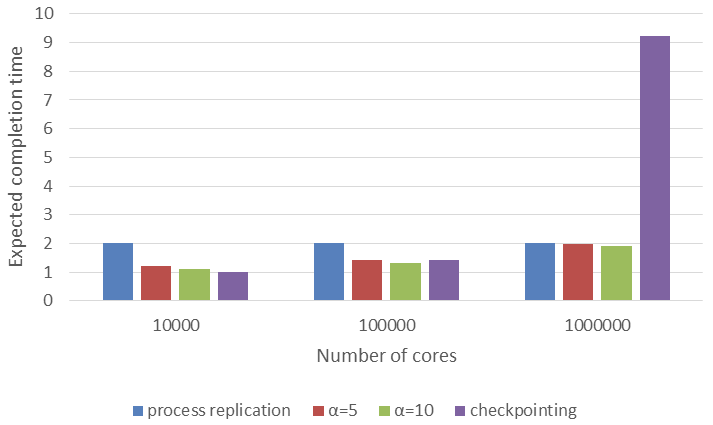
\includegraphics[width=0.70.7\columnwidth]{Figures/nt25}
%		} 
%		\subfigure[Expected energy consumption]
%		{
%			\label{fig:ne25}
%			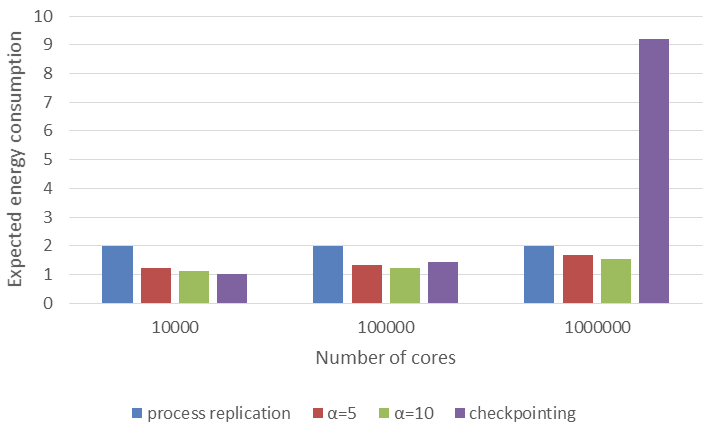
\includegraphics[width=0.70.7\columnwidth]{Figures/ne25}
%		} 
%	\end{center}
%	%\vskip -0.22in 
%	\caption{Sensitivity to number of cores. $W=N$, MTBF=25years, $\rho=0.5$.}
%	\label{fig:n25}
%\end{figure}
